\section{双 Bruhat 胞腔的簇参数化：圈群}

现在把这一构造推广到圈群，即对 $\widehat{\operatorname{PGL}}(N)$ 陈述它。

对圈群，Ad-不变函数有无穷多个，而它们具有有限维的 Poisson 子流形，因此可以构造一类宽得多的可积系统。

与单群情形的主要区别在于：仿射群的嘉当矩阵不可逆，因此关系 (1.3) 与 (1.4) 现在定义的是互不同构的李代数。前者定义中心扩张圈群 $\operatorname{PGL}^{\#}(N)=\widehat{\operatorname{PGL}}(N)\ltimes\C^\times$，后者则对应当余扩张圈群 $\operatorname{PGL}^{\sharp}(N)=\widehat{\operatorname{PGL}}(N)\rtimes\C^\times$；例如见 [15]。为我们的目的，我们使用群 $\operatorname{PGL}^{\sharp}(N)$，因为它允许簇参数化。这个群的单根可以等同于集合 $\Pi=\Z/N\Z$，其 Dynkin 图是一个有 $N$ 个顶点的闭环。

\subsection{余扩张仿射外尔群、绕线与 Thurston 图}

群 $\operatorname{PGL}^{\sharp}(N)$ 的外尔群 $\tilde W$ 也带有一个中心余扩张 $\tilde W^{\sharp}=\tilde W\rtimes\Z/N\Z$，并可由对应于单根 $\{s_i\mid i\in\Z/N\Z\}$ 的生成元以及一个附加生成元 $\Lambda$ 定义，关系为
\begin{equation}\label{eq:1.12}
\begin{gathered}
s_is_{i+1}s_i=s_{i+1}s_is_{i+1},\\
\Lambda s_i=s_{i+1}\Lambda,\\
s_i^2=1,\qquad \Lambda^N=1.
\end{gathered}
\tag{1.12}
\end{equation}
类似地，群 $(\tilde W\times\tilde W)^{\sharp}=(\tilde W\times\tilde W)\rtimes(\Z/N\Z)$ 由 $\{s_i\mid i\in\Pi\cup\bar\Pi\}$（现在对应于正单根或负单根）与 $\Lambda$ 生成，满足 (1.12)，并附加一个关系
\begin{equation}\label{eq:1.13}
s_is_j=s_js_i\quad\text{若 } i>0 \text{ 且 } j<0.
\tag{1.13}
\end{equation}
由 $s_is_{\bar\imath}$ 与 $\Lambda$ 生成的 $(\tilde W\times\tilde W)^{\sharp}$ 的子群，通过显然的同构 $s_is_{\bar\imath}\mapsto s_i$ 同构于 $\tilde W^{\sharp}$。我们把它称为\emph{对角子群}，记作 $\tilde W^{\sharp}_+$。

群 $\tilde W^{\sharp}$ 的元素以及它们分解为生成元之乘积的方式，可以用\emph{绕线图}（wiring diagram）直观地表示，这与 $A_{N-1}$ 型有限外尔群的情形类似，例如见 [7]。唯一的区别是，在仿射情形图要画在柱面上而不是条带上。

一条绕线图是柱面 $\R/N\Z\times[0,1]$ 上的一组 $N$ 条路径 $\gamma_k$，它们把柱面一侧的整数点双射到另一侧的整数点。这些路径按同伦以及保持柱面边界逐点不动的环面微分同胚（即 Dehn 扭转）等同；这条规则保证了关系 $\Lambda^N=1$。群的乘积对应于把一个柱面的右侧与另一个柱面的左侧粘合。生成元 $s_i$ 对应于这样的图：连接第 $i$ 个点与第 $i+1$ 个点的路径、连接第 $i+1$ 个点与第 $i$ 个点的路径各有一个交点，其余路径保持水平。生成元 $\Lambda$ 对应的图把第 $i$ 个点连到第 $i+1$ 个点，对任意 $i$ 皆然（见图 1.3）。

反之，给定一个只有二重交点、且路径从左到右单调的绕线图，可以如下给它联系一个 $\tilde W^{\sharp}$ 中的词。用一条线把柱面剪开成矩形：这条线从柱面左侧出发（起点在第 $(N-1\ (\mathrm{mod}\ N))$ 个点与第 $(0\ (\mathrm{mod}\ N))$ 个点之间）走到右侧，并且对它所穿过的图的每个面，它都从该面的最左点进入、从最右点离开。剪开后，每个交点都像有限条带图那样给出生成元 $s_i$；落在剪开线上的交点另外给出生成元 $s_0$。余扩张生成元 $\Lambda$ 的幂，由剪开线与柱面右侧相交于哪一段决定。

余扩张同态 $\tilde W^{\sharp}\to\Z/N\Z$ 也可以描述为图与柱面的一条生成元的相交指数：把所有路径从左到右定向，数它们与一条同样从左到右、避开整数点的水平直线按定向计数的交点数。计算这个余扩张还有一种方法：对每条路径联系一个整数，度量路径两端在柱面的万有覆盖上坐标之差。这些数之和除以 $N$ 再模 $N$ 就是所求同态。容易验证，这个和总能被 $N$ 整除，并且在 Dehn 扭转下模 $N^2$ 不变。

要表示群 $(\tilde W\times\tilde W)^{\sharp}$ 的元素，只需给出两个绕线图，每个 $\tilde W$ 的拷贝一个，它们有相同的线数和相同的余扩张。然而，要把这个群的某个具体分解表示成生成元之乘积，我们使用 Thurston 图（见附录 1.12）：它由对应于两个 $W$ 因子的两个绕线图画在同一个柱面上构成，第二个相对第一个略向下移，并附加两个条件：(1) 每条竖线交替地与两份图的线相交；(2) 于是所有交点必为三重点；(3) 对应于第一份（相应地第二份）图的线从左到右（相应地从右到左）定向，见图 1.4 C。因此三重点有两类：第一份图的两条线与第二份图的一条线相交，及其反向；它们分别对应于生成元 $s_i$（$i>0$）与 $i<0$。

下面我们把柱面图画在矩形上，并约定矩形的下边与上边等同。

\begin{figure}[htbp]
\centering
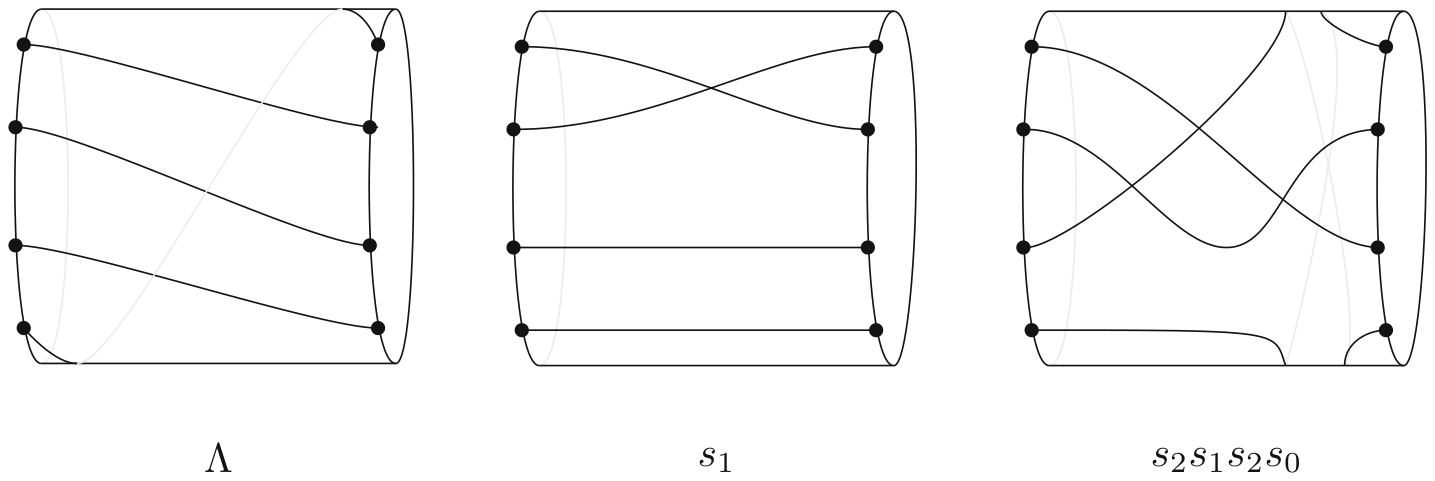
\includegraphics[width=378.8pt]{figs/f1-03.png}
\caption{余扩张仿射外尔群元素的柱面图。}
\label{fig:1.3}
\end{figure}

\subsection{余扩张圈群的实现}

我们将使用群 $\operatorname{PGL}^{\sharp}(N)$ 的两种不同实现：无穷矩阵实现与圈实现。在无穷矩阵实现中，它可以等同于无穷矩阵 $\{A^J_I\mid I,J\in\Z\}$ 的群，模去乘以常数，并满足以下两个条件：
\begin{equation}\label{eq:1.14}
\begin{gathered}
A^J_I=0\quad\text{对 } |I-J|\gg 0,\\
A^{J+N}_{I+N}=x\,A^J_I\quad\text{对某个 } x\in\C^\times.
\end{gathered}
\tag{1.14}
\end{equation}
在 Laurent 实现中，群 $\operatorname{PGL}^{\sharp}(N)$ 可以等同于形如 $A(\lambda)T_x$ 的表达式之群，其中 $T_x$ 是乘以 $x$ 的乘法平移算子，
\begin{equation}\label{eq:1.15}
T_x=\exp\left(\log x\,\lambda\frac{\partial}{\partial\lambda}\right)=x^{\lambda\partial/\partial\lambda},
\tag{1.15}
\end{equation}
而 $A(\lambda)$ 是取值于 $N\times N$ 矩阵的 Laurent 多项式，同样模去乘以常数。因此这类表达式的乘法规则是
\begin{equation}\label{eq:1.16}
A_1(\lambda)T_{x_1}\cdot A_2(\lambda)T_{x_2}=A_1(\lambda)A_2(x_1\lambda)T_{x_1x_2}.
\tag{1.16}
\end{equation}

无穷矩阵实现与圈实现之间的对应由同构
\[
A^J_I\mapsto\sum_{K\in\Z}A^{J+KN}_I\lambda^KT_x,
\]
给出，其中右边 $I,J\in1,\dots,N$，$x$ 是条件 (1.14) 中的准周期因子。

圈群 $\operatorname{PGL}^{\sharp}(N)$ 除了 $\operatorname{PGL}(N)$ 的生成元之外，还多出一组生成元，记作 $E_0$、$E_{\bar0}$ 与 $H_0(x)$。在圈实现中，$i\neq0,\bar0$ 的矩阵 $E_i$ 与相应的有限维群 $\operatorname{PGL}(N)$ 的矩阵相同，而矩阵 $H_i(x)$ 要乘以 $T_x$，即
\begin{equation}\label{eq:1.17}
H_i(x)=
\begin{pmatrix}
x&0&\cdots&&0\\
0&\ddots&&&&\\
\vdots&&x&&&\\
&&&1&\ddots&\\
&&&&\ddots&0\\
0&&&&&1
\end{pmatrix}T_x,
\qquad
E_i=
\begin{pmatrix}
1&0&\cdots&&0\\
0&\ddots&&&&\\
\vdots&&1&1&&\\
&&&&\ddots&0\\
0&&&&&1
\end{pmatrix},
\tag{1.17}
\end{equation}
其中对 $i>0$，$E_i=E_{\bar\imath}^{\mathrm{tr}}$。此外，对 $i=0$ 有 $H_0(x)=T_x$，以及
\begin{equation}\label{eq:1.18}
E_0=
\begin{pmatrix}
1&0&\cdots&0\\
\vdots&\ddots&&\vdots\\
0&&\ddots&0\\
\lambda&\cdots&0&1
\end{pmatrix},
\qquad
E_{\bar0}=
\begin{pmatrix}
1&0&\cdots&\lambda^{-1}\\
\vdots&\ddots&&\vdots\\
0&&\ddots&0\\
0&\cdots&0&1
\end{pmatrix}.
\tag{1.18}
\end{equation}
再引入元素 $\Lambda\in\widehat{\operatorname{PGL}}(N)$ 也是有用的，它在无穷矩阵实现中为 $\Lambda^J_I=\delta^{J+1}_I$，在圈实现中为
\begin{equation}\label{eq:1.19}
\Lambda=
\begin{pmatrix}
0&1&\cdots&0\\
\vdots&\ddots&\ddots&\vdots\\
0&\cdots&0&1\\
\lambda&\cdots&0&0
\end{pmatrix}.
\tag{1.19}
\end{equation}
这个矩阵满足
\begin{equation}\label{eq:1.20}
\Lambda E_i\Lambda^{-1}=E_{i+1},\qquad
\Lambda H_i(z)\Lambda^{-1}=H_{i+1}(z),\qquad i\in\Z/N\Z,
\tag{1.20}
\end{equation}
即算子 $\Lambda$ 沿 $\widehat{\operatorname{PGL}}(N)$ 的 Dynkin 图作用为平移一个单位。

\begin{figure}[htbp]
\centering
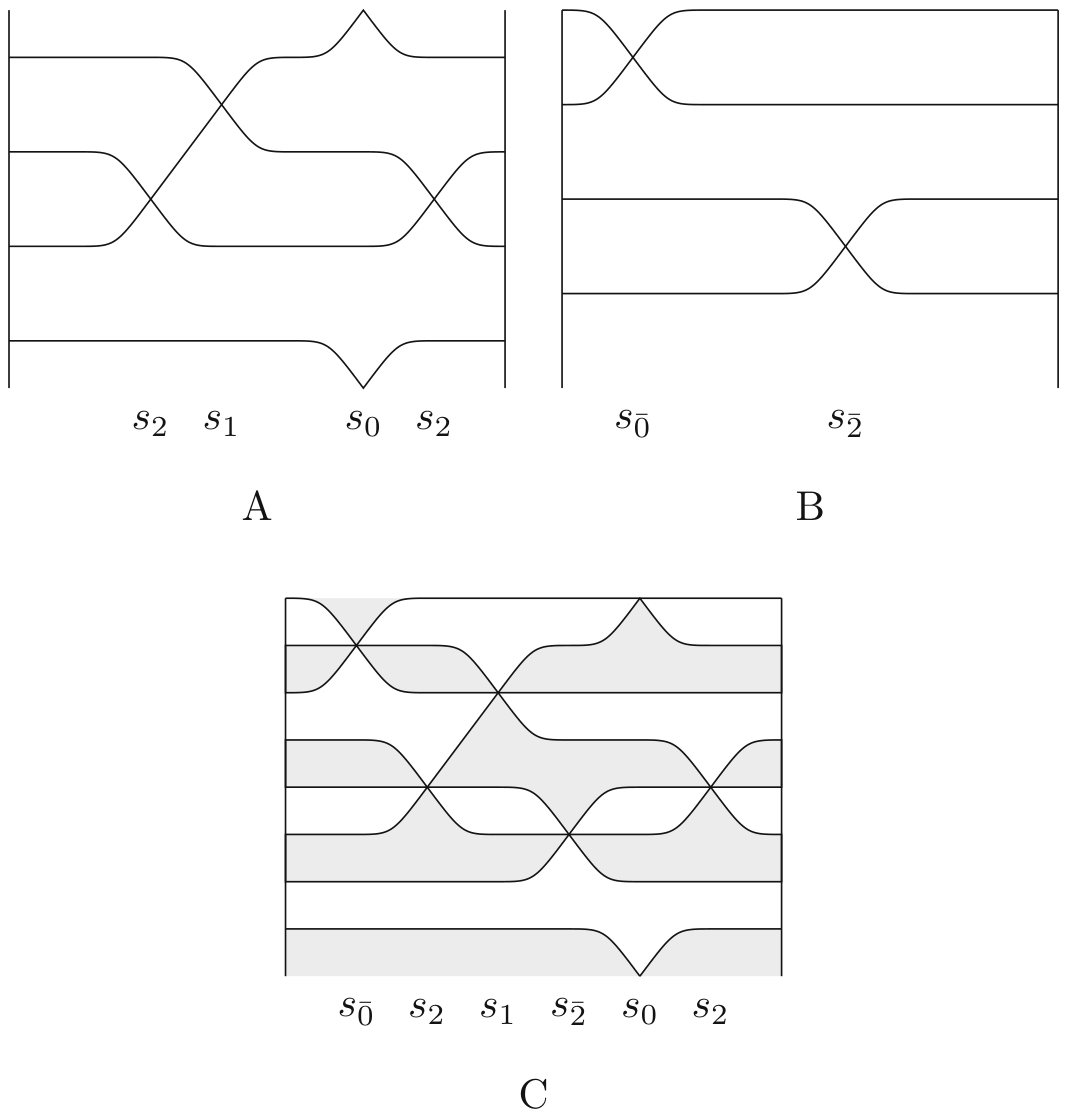
\includegraphics[width=281.7pt]{figs/f1-04.png}
\caption{A：绕线图；B：群 $W$ 的第二个拷贝的绕线图；C：Thurston 图。}
\label{fig:1.4}
\end{figure}

\subsection{双 Bruhat 胞腔上的可积系统}

\begin{figure}[htbp]
\centering
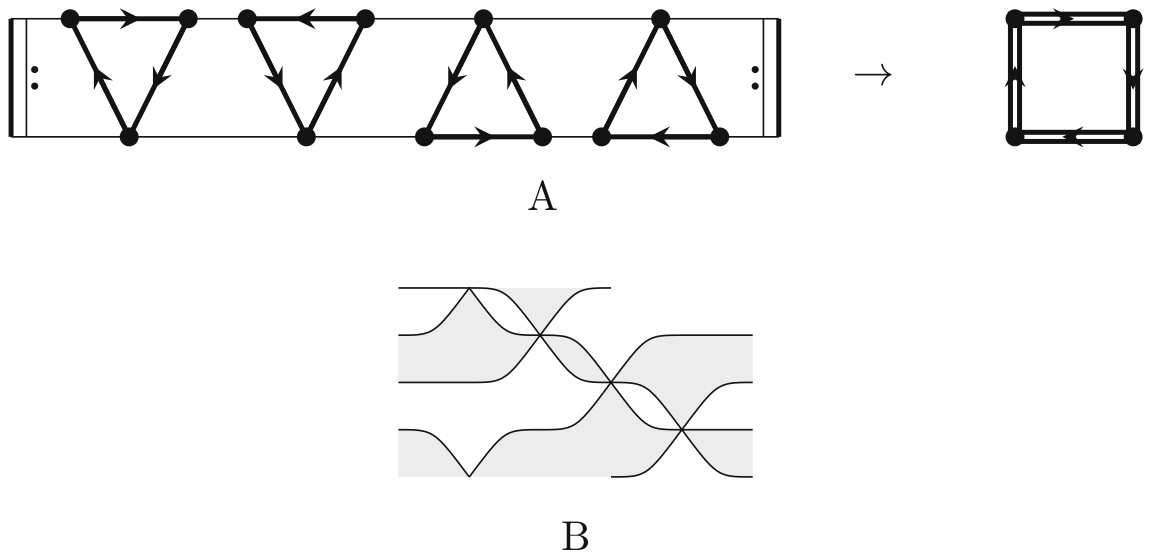
\includegraphics[width=304.1pt]{figs/f1-05.png}
\caption{胞腔 $\widehat{\operatorname{PGL}}^{\sharp}(2)/\mathrm{Ad}H$ 的图，对应词 $0\bar01\bar1$。A：交换图；B：Thurston 图。}
\label{fig:1.5}
\end{figure}

仿射李群的外尔群是无穷的（例如所有生成元之积具有无穷阶），因此与有限维情形不同，可以考虑任意长的词，它们对应于维数任意大的 Poisson 子流形。$\operatorname{PGL}^{\sharp}(N)$ 上的 Ad-不变函数空间是有限生成的，但在其子群 $\widehat{\operatorname{PGL}}(N)$ 上是无穷生成的。

圈群 $\widehat{\operatorname{PGL}}(N)^{\sharp}$ 的双 Bruhat 胞腔的簇参数化完全沿着我们对单群的路线进行。在交换图（见附录 1.11）层面唯一的区别是应当多添一条线；$u=0\bar01\bar1$ 的交换图例子见图 1.5 A。$\hat G_u$ 的 Thurston 图画在带左右边界的柱面上，以取代单群情形下的无限条带；而 $\hat G_u/\mathrm{Ad}H$ 的 Thurston 图画在环面上，把柱面的左边界与右边界粘合即得（即在图 1.5 B 中应把上边与下边、左边与右边分别等同）。

设 $u=s_{i_1}\cdots s_{i_n}\Lambda^k$ 是 $u\in(\tilde W\times\tilde W)^{\sharp}$ 的任意约化分解。相应的双 Bruhat 胞腔可以用 $n$ 个变量 $x=(x_1,\dots,x_n)$ 通过下述公式参数化：
\begin{equation}\label{eq:1.21}
(x_1,\dots,x_n)\mapsto A(\lambda,x)=H_{i_1}(x_1)E_{i_1}\cdots H_{i_n}(x_n)E_{i_n}\Lambda^k.
\tag{1.21}
\end{equation}
为了得到 $\widehat{\operatorname{PGL}}(N)/\mathrm{Ad}H$ 而非 $\operatorname{PGL}^{\sharp}(N)/\mathrm{Ad}H$ 的元素，需要在 (1.21) 中要求
\begin{equation}\label{eq:1.22}
\prod_j x_j=1.
\tag{1.22}
\end{equation}
若此条件满足，矩阵 $A(\lambda,x)$ 就是一个元素为 Laurent 多项式的矩阵，但定义到乘以常数 $\alpha$ 以及平移 $\lambda\to\beta\lambda$（这不过是它被 $H_0(\beta)=T_\beta$ 共轭的结果）为止。

考虑函数
\begin{equation}\label{eq:1.23}
S_{s_{i_1},\dots,s_{i_n}\Lambda^k}(\lambda,\mu,x)=\det(A(\lambda,x)-\mu)),
\tag{1.23}
\end{equation}
我们称它为可积模型的\emph{生成函数}。由于上述不确定性，这个函数定义得不好。然而，若认为它定义到一个变换
\[
S_{s_{i_1},\dots,s_{i_n}\Lambda^k}(\lambda,\mu,x)\simeq\alpha S_{s_{i_1},\dots,s_{i_n}\Lambda^k}(\beta\lambda,\gamma\mu,x)
\]
为止——其中 $\alpha$、$\beta$、$\gamma$ 是 $x_1,\dots,x_n$ 的任意函数——它就已经定义良好了。

计算 (1.23) 中的行列式，该函数表示为 $\lambda$ 与 $\mu$ 的 Laurent 多项式，
\begin{equation}\label{eq:1.24}
S_{s_{i_1},\dots,s_{i_n}\Lambda^k}(\lambda,\mu,x)=\sum_{i,j}H_{ij}(x)\lambda^i\mu^j.
\tag{1.24}
\end{equation}
记 $\Delta$ 为 (1.24) 的 Newton 多边形，即平面上使 $H_{ij}(x)\neq0$ 的点 $(i,j)$ 的凸包。固定 $\Delta$ 的任意三个顶点，调整 $\alpha$、$\beta$、$\gamma$ 使相应的系数 $H_{ij}$ 等于 $1$；所得的配分函数称为\emph{归一化的}。

\begin{theorem}\label{thm:1.4.1}
归一化配分函数的展开 (1.24) 的系数 $\{H_{ij}(x)\}$ 恰是 Poisson 子流形 $\hat G_{s_{i_1},\dots,\allowbreak s_{i_n}\Lambda^k}/\mathrm{Ad}H$ 上定义良好的 Ad-不变函数，因此它们彼此 Poisson 交换。
\end{theorem}

证明它们确实构成可积系统的运动积分集合，以及讨论这个系统的性质，将在我们建立这些系统与 Goncharov–Kenyon 可积系统的同构之后进行。
